In the analysis, BSM signals~\ttH~are used to interpret both~\ttH~and~\ttA~assuming the kinematics are similar. In the following, the comparison between $t\bar{t}H$ and $t\bar{t}A$ is shown. In addition, BSM signals $t\bar{t}H$ contain only the $s$-channel diagrams, and the missing $t$-channel of BSM signals are also studied in the following. Figure \ref{fig:bsm_diagrams} shows the $s$-channel and $t$-channel diagrams. 

The BSM signal samples are produced with AthGeneration, 21.6.39.1 and same parameter cards as existing signal samples. In total, 0.5 million events are produced for each process and mass point.  The estimated cross-sections for the \ttH production in the $s$-channel, $t$-channel and $s$+$t$ channel is shown in Figure~\ref{fig:cross-section} with each value estimated using 10000 events. 


Kinematics are checked with rivet-3. The truth objects are found in the generator level, with following object selection:
\begin{itemize}
  \item Electron and muon: $\pT > 10$ GeV and $|\eta| < 2.5$
    \item Jet: $\pT >25$ GeV and $|\eta| < 2.5$
      \item Hadronic tau is counted in the jet collection with same $\pT >25$ GeV and $|\eta| < 2.5$ selection (same as setup for our analysis)
        \item Leptonic tau is decayed into electron or muon, which are counted in the electron or muon collections
          \item $\HT$ is calculated with leptons (electrons \& muons) and jets. No selection on $\HT$.
\end{itemize}


The inclusive region is defined with object selection shown above. The kinematics with different mass points in the inclusive region are shown in Figures \ref{Fig:t_channel_400}-\ref{Fig:t_channel_1000}. Around 10-20\% difference is observed between $t\bar{t}H$ and $t\bar{t}A$ samples at low mass points ($\mH=400$ GeV-$\mH=600$ GeV), and the region with larger difference are with less statistics. Around 10\% difference between $s$-channel and $s$+$t$-channel on $\HT$ for $\mH=400$ GeV. 



% TODO: \usepackage{graphicx} required
\begin{figure}[htbp!] 
  \centering
  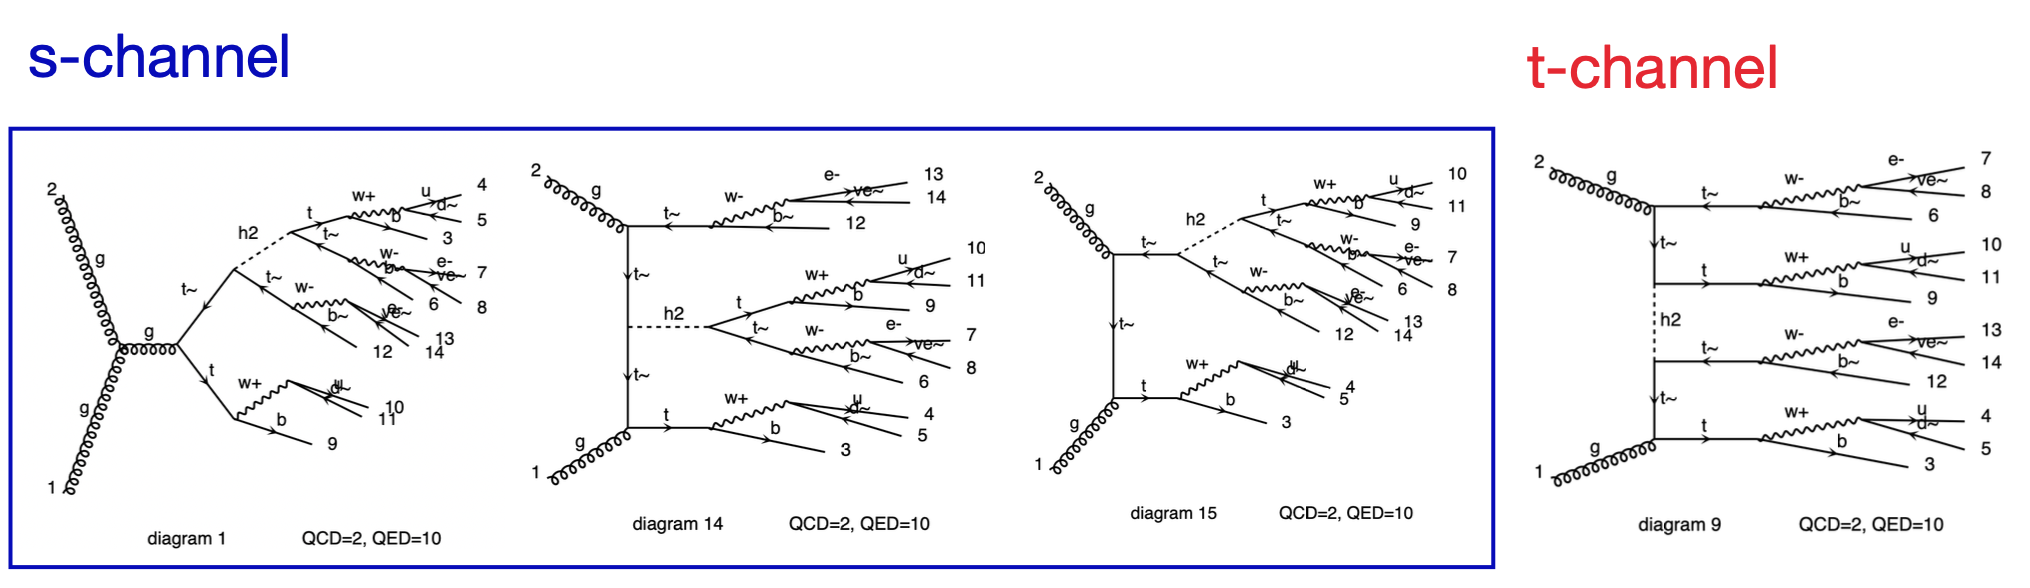
\includegraphics[width=0.9\linewidth]{figures/signal_modeling/t_channel/diagrams}
  \caption{Feynman diagrams of $s$-channel and $t$-channel for BSM signals.}
  \label{fig:bsm_diagrams}
\end{figure}


% TODO: \usepackage{graphicx} required
\begin{figure}[htbp!] 
  \centering
  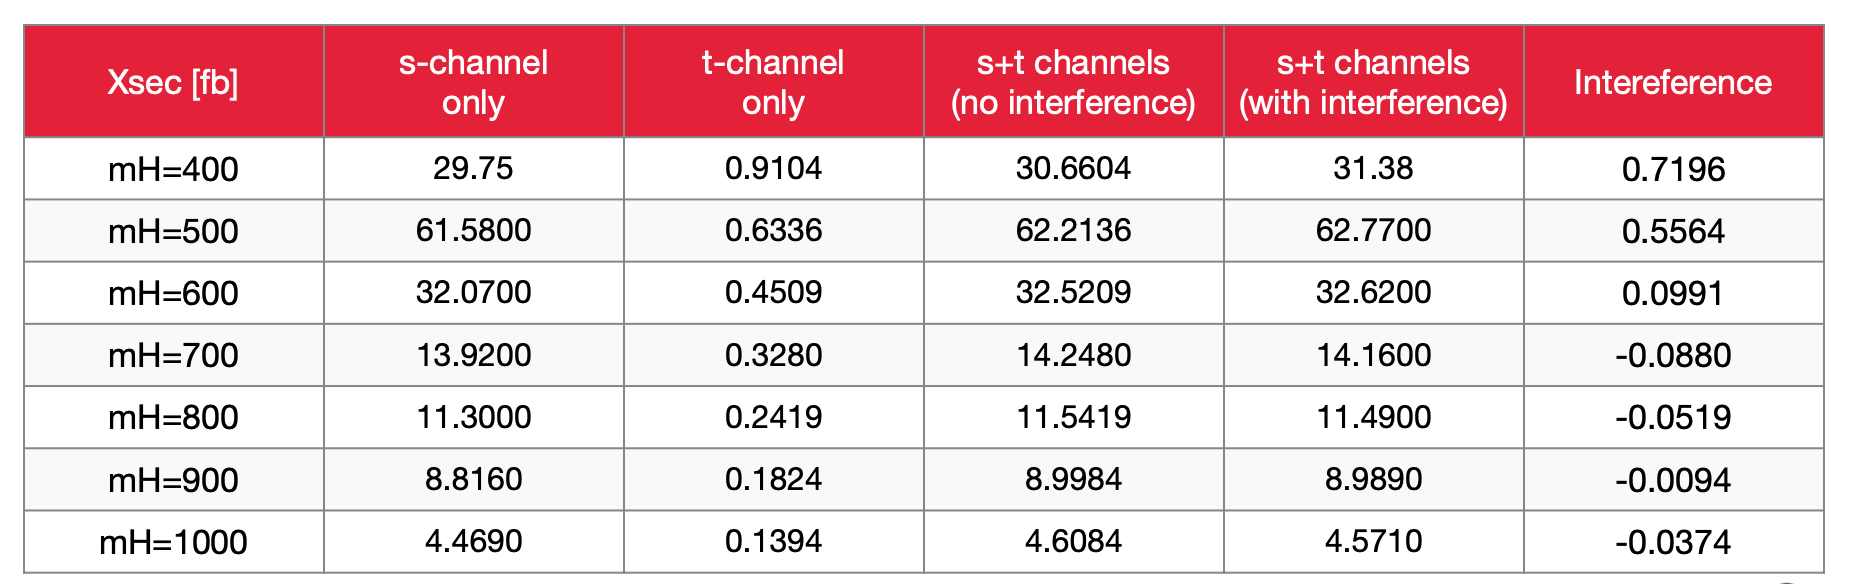
\includegraphics[width=0.9\linewidth]{figures/signal_modeling/t_channel/cross-section}
  \caption{Estimated cross-section for the \ttH production in the  $s$-channel, $t$-channel and $s$+$t$ channel. Each value is estimated with 10000 events. Filter efficiencies are about 80\% but they are not applied in the table.}
  \label{fig:cross-section}
\end{figure}

\begin{figure}[htbp!]
  \begin{minipage}{0.33\textwidth}
    \centering
    
\includegraphics[width=0.9\linewidth]{figures/signal_modeling/HA_difference/Results_m400_w5/Event_Inclusive_HT_normed}
    \end{minipage}
  \begin{minipage}{0.33\textwidth}
    \centering
    
\includegraphics[width=0.9\linewidth]{figures/signal_modeling/HA_difference/Results_m400_w5/Event_Inclusive_HT_jets_normed}
    \end{minipage}
  \begin{minipage}{0.33\textwidth}
    \centering
    
\includegraphics[width=0.9\linewidth]{figures/signal_modeling/HA_difference/Results_m400_w5/Event_Inclusive_nJets_normed}
    \end{minipage}
  \begin{minipage}{0.33\textwidth}
    \centering
    
\includegraphics[width=0.9\linewidth]{figures/signal_modeling/HA_difference/Results_m400_w5/Event_Inclusive_nBjets_normed}
    \end{minipage}
  \begin{minipage}{0.33\textwidth}
    \centering
    
\includegraphics[width=0.9\linewidth]{figures/signal_modeling/HA_difference/Results_m400_w5/Event_Inclusive_jet0Pt_normed}
    \end{minipage}
  \begin{minipage}{0.33\textwidth}
    \centering
    
\includegraphics[width=0.9\linewidth]{figures/signal_modeling/HA_difference/Results_m400_w5/Event_Inclusive_jet0Eta_normed}
    \end{minipage}
  \begin{minipage}{0.33\textwidth}
    \centering
    
\includegraphics[width=0.9\linewidth]{figures/signal_modeling/HA_difference/Results_m400_w5/Event_Inclusive_lep0Pt_normed}
    \end{minipage}
  \begin{minipage}{0.33\textwidth}
    \centering
    
\includegraphics[width=0.9\linewidth]{figures/signal_modeling/HA_difference/Results_m400_w5/Event_Inclusive_lep0Eta_normed}
    \end{minipage}

  \caption{\label{Fig:t_channel_400}Kinematic comparison between $t\bar{t}H$ and $t\bar{t}A$ production in the $s$-channel and $s$+$t$-channel for $\mH=400$~GeV in the inclusive region. The shapes are normalised to unit.}

\end{figure}

\begin{figure}[htbp!]
  \begin{minipage}{0.33\textwidth}
    \centering
    
\includegraphics[width=0.9\linewidth]{figures/signal_modeling/HA_difference/Results_m500_w5/Event_Inclusive_HT_normed}
    \end{minipage}
  \begin{minipage}{0.33\textwidth}
    \centering
    
\includegraphics[width=0.9\linewidth]{figures/signal_modeling/HA_difference/Results_m500_w5/Event_Inclusive_HT_jets_normed}
    \end{minipage}
  \begin{minipage}{0.33\textwidth}
    \centering
    
\includegraphics[width=0.9\linewidth]{figures/signal_modeling/HA_difference/Results_m500_w5/Event_Inclusive_nJets_normed}
    \end{minipage}
  \begin{minipage}{0.33\textwidth}
    \centering
    
\includegraphics[width=0.9\linewidth]{figures/signal_modeling/HA_difference/Results_m500_w5/Event_Inclusive_nBjets_normed}
    \end{minipage}
  \begin{minipage}{0.33\textwidth}
    \centering
    
\includegraphics[width=0.9\linewidth]{figures/signal_modeling/HA_difference/Results_m500_w5/Event_Inclusive_jet0Pt_normed}
    \end{minipage}
  \begin{minipage}{0.33\textwidth}
    \centering
    
\includegraphics[width=0.9\linewidth]{figures/signal_modeling/HA_difference/Results_m500_w5/Event_Inclusive_jet0Eta_normed}
    \end{minipage}
  \begin{minipage}{0.33\textwidth}
    \centering
    
\includegraphics[width=0.9\linewidth]{figures/signal_modeling/HA_difference/Results_m500_w5/Event_Inclusive_lep0Pt_normed}
    \end{minipage}
  \begin{minipage}{0.33\textwidth}
    \centering
    
\includegraphics[width=0.9\linewidth]{figures/signal_modeling/HA_difference/Results_m500_w5/Event_Inclusive_lep0Eta_normed}
    \end{minipage}

  \caption{\label{Fig:t_channel_500}Kinematic comparison between $t\bar{t}H$ and $t\bar{t}A$ production in the $s$-channel and $s$+$t$-channel for$\mH=500$~GeV in the inclusive region. The shapes are normalised to unit.}

\end{figure}

\begin{figure}[htbp!]
  \begin{minipage}{0.33\textwidth}
    \centering
    
\includegraphics[width=0.9\linewidth]{figures/signal_modeling/HA_difference/Results_m600_w10/Event_Inclusive_HT_normed}
    \end{minipage}
  \begin{minipage}{0.33\textwidth}
    \centering
    
\includegraphics[width=0.9\linewidth]{figures/signal_modeling/HA_difference/Results_m600_w10/Event_Inclusive_HT_jets_normed}
    \end{minipage}
  \begin{minipage}{0.33\textwidth}
    \centering
    
\includegraphics[width=0.9\linewidth]{figures/signal_modeling/HA_difference/Results_m600_w10/Event_Inclusive_nJets_normed}
    \end{minipage}
  \begin{minipage}{0.33\textwidth}
    \centering
    
\includegraphics[width=0.9\linewidth]{figures/signal_modeling/HA_difference/Results_m600_w10/Event_Inclusive_nBjets_normed}
    \end{minipage}
  \begin{minipage}{0.33\textwidth}
    \centering
    
\includegraphics[width=0.9\linewidth]{figures/signal_modeling/HA_difference/Results_m600_w10/Event_Inclusive_jet0Pt_normed}
    \end{minipage}
  \begin{minipage}{0.33\textwidth}
    \centering
    
\includegraphics[width=0.9\linewidth]{figures/signal_modeling/HA_difference/Results_m600_w10/Event_Inclusive_jet0Eta_normed}
    \end{minipage}
  \begin{minipage}{0.33\textwidth}
    \centering
    
\includegraphics[width=0.9\linewidth]{figures/signal_modeling/HA_difference/Results_m600_w10/Event_Inclusive_lep0Pt_normed}
    \end{minipage}
  \begin{minipage}{0.33\textwidth}
    \centering
    
\includegraphics[width=0.9\linewidth]{figures/signal_modeling/HA_difference/Results_m600_w10/Event_Inclusive_lep0Eta_normed}
    \end{minipage}
  

  \caption{\label{Fig:t_channel_600}Kinematic comparison between $t\bar{t}H$ and $t\bar{t}A$ production in the $s$-channel and $s$+$t$-channel for $\mH=600$~GeV in the inclusive region. The shapes are normalised to unit.}

\end{figure}

\begin{figure}[htbp!]
  \begin{minipage}{0.33\textwidth}
    \centering
    
\includegraphics[width=0.9\linewidth]{figures/signal_modeling/HA_difference/Results_m700_w20/Event_Inclusive_HT_normed}
    \end{minipage}
  \begin{minipage}{0.33\textwidth}
    \centering
    
\includegraphics[width=0.9\linewidth]{figures/signal_modeling/HA_difference/Results_m700_w20/Event_Inclusive_HT_jets_normed}
    \end{minipage}
  \begin{minipage}{0.33\textwidth}
    \centering
    
\includegraphics[width=0.9\linewidth]{figures/signal_modeling/HA_difference/Results_m700_w20/Event_Inclusive_nJets_normed}
    \end{minipage}
  \begin{minipage}{0.33\textwidth}
    \centering
    
\includegraphics[width=0.9\linewidth]{figures/signal_modeling/HA_difference/Results_m700_w20/Event_Inclusive_nBjets_normed}
    \end{minipage}
  \begin{minipage}{0.33\textwidth}
    \centering
    
\includegraphics[width=0.9\linewidth]{figures/signal_modeling/HA_difference/Results_m700_w20/Event_Inclusive_jet0Pt_normed}
    \end{minipage}
  \begin{minipage}{0.33\textwidth}
    \centering
    
\includegraphics[width=0.9\linewidth]{figures/signal_modeling/HA_difference/Results_m700_w20/Event_Inclusive_jet0Eta_normed}
    \end{minipage}
  \begin{minipage}{0.33\textwidth}
    \centering
    
\includegraphics[width=0.9\linewidth]{figures/signal_modeling/HA_difference/Results_m700_w20/Event_Inclusive_lep0Pt_normed}
    \end{minipage}
  \begin{minipage}{0.33\textwidth}
    \centering
    
\includegraphics[width=0.9\linewidth]{figures/signal_modeling/HA_difference/Results_m700_w20/Event_Inclusive_lep0Eta_normed}
    \end{minipage}
  

  \caption{\label{Fig:t_channel_700}Kinematic comparison between $t\bar{t}H$ and $t\bar{t}A$ production in the $s$-channel and $s$+$t$-channel for $\mH=700$~GeV in the inclusive region. The shapes are normalised to unit.}

\end{figure}

\begin{figure}[htbp!]
  \begin{minipage}{0.33\textwidth}
    \centering
    
\includegraphics[width=0.9\linewidth]{figures/signal_modeling/HA_difference/Results_m800_w20/Event_Inclusive_HT_normed}
    \end{minipage}
  \begin{minipage}{0.33\textwidth}
    \centering
    
\includegraphics[width=0.9\linewidth]{figures/signal_modeling/HA_difference/Results_m800_w20/Event_Inclusive_HT_jets_normed}
    \end{minipage}
  \begin{minipage}{0.33\textwidth}
    \centering
    
\includegraphics[width=0.9\linewidth]{figures/signal_modeling/HA_difference/Results_m800_w20/Event_Inclusive_nJets_normed}
    \end{minipage}
  \begin{minipage}{0.33\textwidth}
    \centering
    
\includegraphics[width=0.9\linewidth]{figures/signal_modeling/HA_difference/Results_m800_w20/Event_Inclusive_nBjets_normed}
    \end{minipage}
  \begin{minipage}{0.33\textwidth}
    \centering
    
\includegraphics[width=0.9\linewidth]{figures/signal_modeling/HA_difference/Results_m800_w20/Event_Inclusive_jet0Pt_normed}
    \end{minipage}
  \begin{minipage}{0.33\textwidth}
    \centering
    
\includegraphics[width=0.9\linewidth]{figures/signal_modeling/HA_difference/Results_m800_w20/Event_Inclusive_jet0Eta_normed}
    \end{minipage}
  \begin{minipage}{0.33\textwidth}
    \centering
    
\includegraphics[width=0.9\linewidth]{figures/signal_modeling/HA_difference/Results_m800_w20/Event_Inclusive_lep0Pt_normed}
    \end{minipage}
  \begin{minipage}{0.33\textwidth}
    \centering
    
\includegraphics[width=0.9\linewidth]{figures/signal_modeling/HA_difference/Results_m800_w20/Event_Inclusive_lep0Eta_normed}
    \end{minipage}
  
  \caption{\label{Fig:t_channel_800}Kinematic comparison between $t\bar{t}H$ and $t\bar{t}A$ production in the $s$-channel and $s$+$t$-channel for $\mH=800$~GeV in the inclusive region. The shapes are normalised to unit.}

\end{figure}

\begin{figure}[htbp!]
  \begin{minipage}{0.33\textwidth}
    \centering
    
\includegraphics[width=0.9\linewidth]{figures/signal_modeling/HA_difference/Results_m900_w20/Event_Inclusive_HT_normed}
    \end{minipage}
  \begin{minipage}{0.33\textwidth}
    \centering
    
\includegraphics[width=0.9\linewidth]{figures/signal_modeling/HA_difference/Results_m900_w20/Event_Inclusive_HT_jets_normed}
    \end{minipage}
  \begin{minipage}{0.33\textwidth}
    \centering
    
\includegraphics[width=0.9\linewidth]{figures/signal_modeling/HA_difference/Results_m900_w20/Event_Inclusive_nJets_normed}
    \end{minipage}
  \begin{minipage}{0.33\textwidth}
    \centering
    
\includegraphics[width=0.9\linewidth]{figures/signal_modeling/HA_difference/Results_m900_w20/Event_Inclusive_nBjets_normed}
    \end{minipage}
  \begin{minipage}{0.33\textwidth}
    \centering
    
\includegraphics[width=0.9\linewidth]{figures/signal_modeling/HA_difference/Results_m900_w20/Event_Inclusive_jet0Pt_normed}
    \end{minipage}
  \begin{minipage}{0.33\textwidth}
    \centering
    
\includegraphics[width=0.9\linewidth]{figures/signal_modeling/HA_difference/Results_m900_w20/Event_Inclusive_jet0Eta_normed}
    \end{minipage}
  \begin{minipage}{0.33\textwidth}
    \centering
    
\includegraphics[width=0.9\linewidth]{figures/signal_modeling/HA_difference/Results_m900_w20/Event_Inclusive_lep0Pt_normed}
    \end{minipage}
  \begin{minipage}{0.33\textwidth}
    \centering
    
\includegraphics[width=0.9\linewidth]{figures/signal_modeling/HA_difference/Results_m900_w20/Event_Inclusive_lep0Eta_normed}
    \end{minipage}
  

  \caption{\label{Fig:t_channel_900}Kinematic comparison between $t\bar{t}H$ and $t\bar{t}A$ production in the $s$-channel and $s$+$t$-channel for $\mH=900$~GeV in the inclusive region. The shapes are normalised to unit.}

\end{figure}

\begin{figure}[htbp!]
  \begin{minipage}{0.33\textwidth}
    \centering
    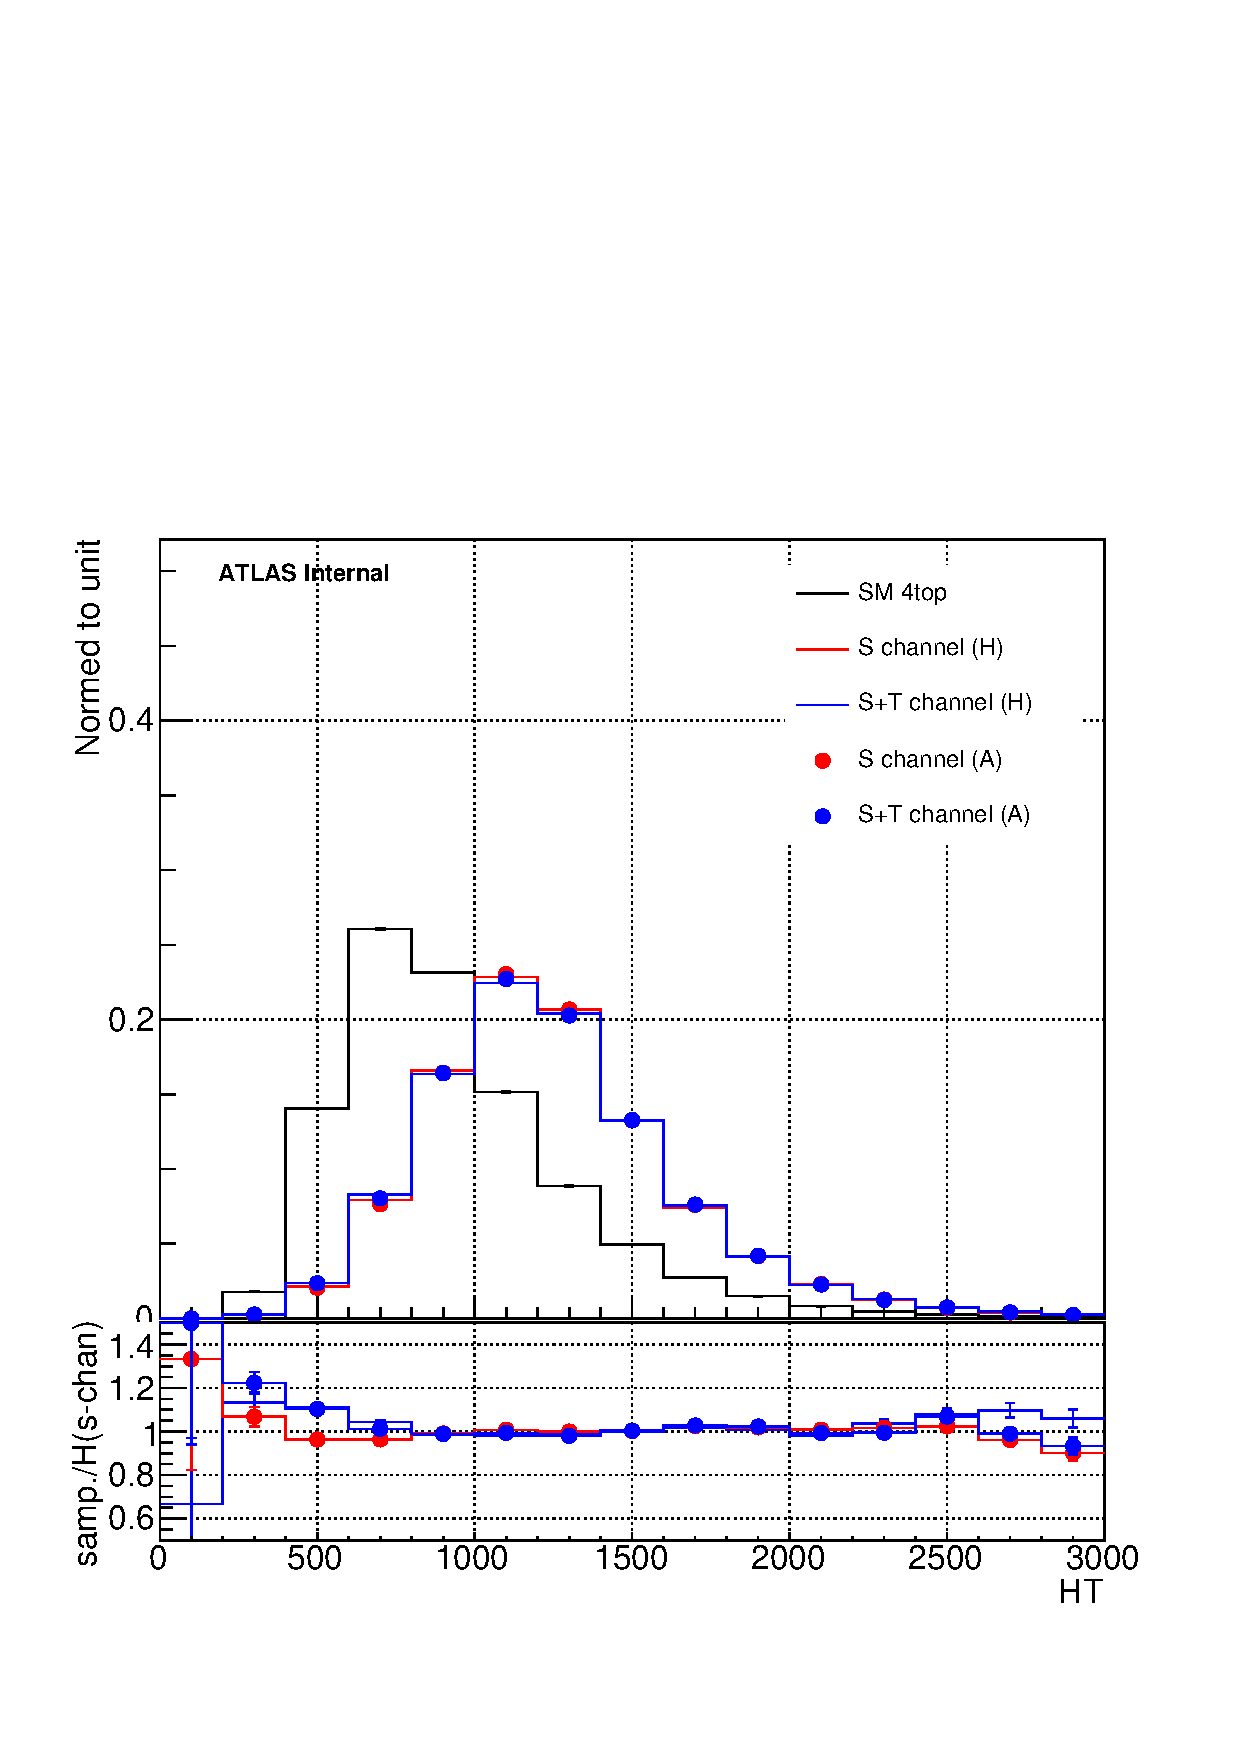
\includegraphics[width=0.9\linewidth]{figures/signal_modeling/HA_difference/Results_m1000_w30/Event_Inclusive_HT_normed}
    \end{minipage}
  \begin{minipage}{0.33\textwidth}
    \centering
    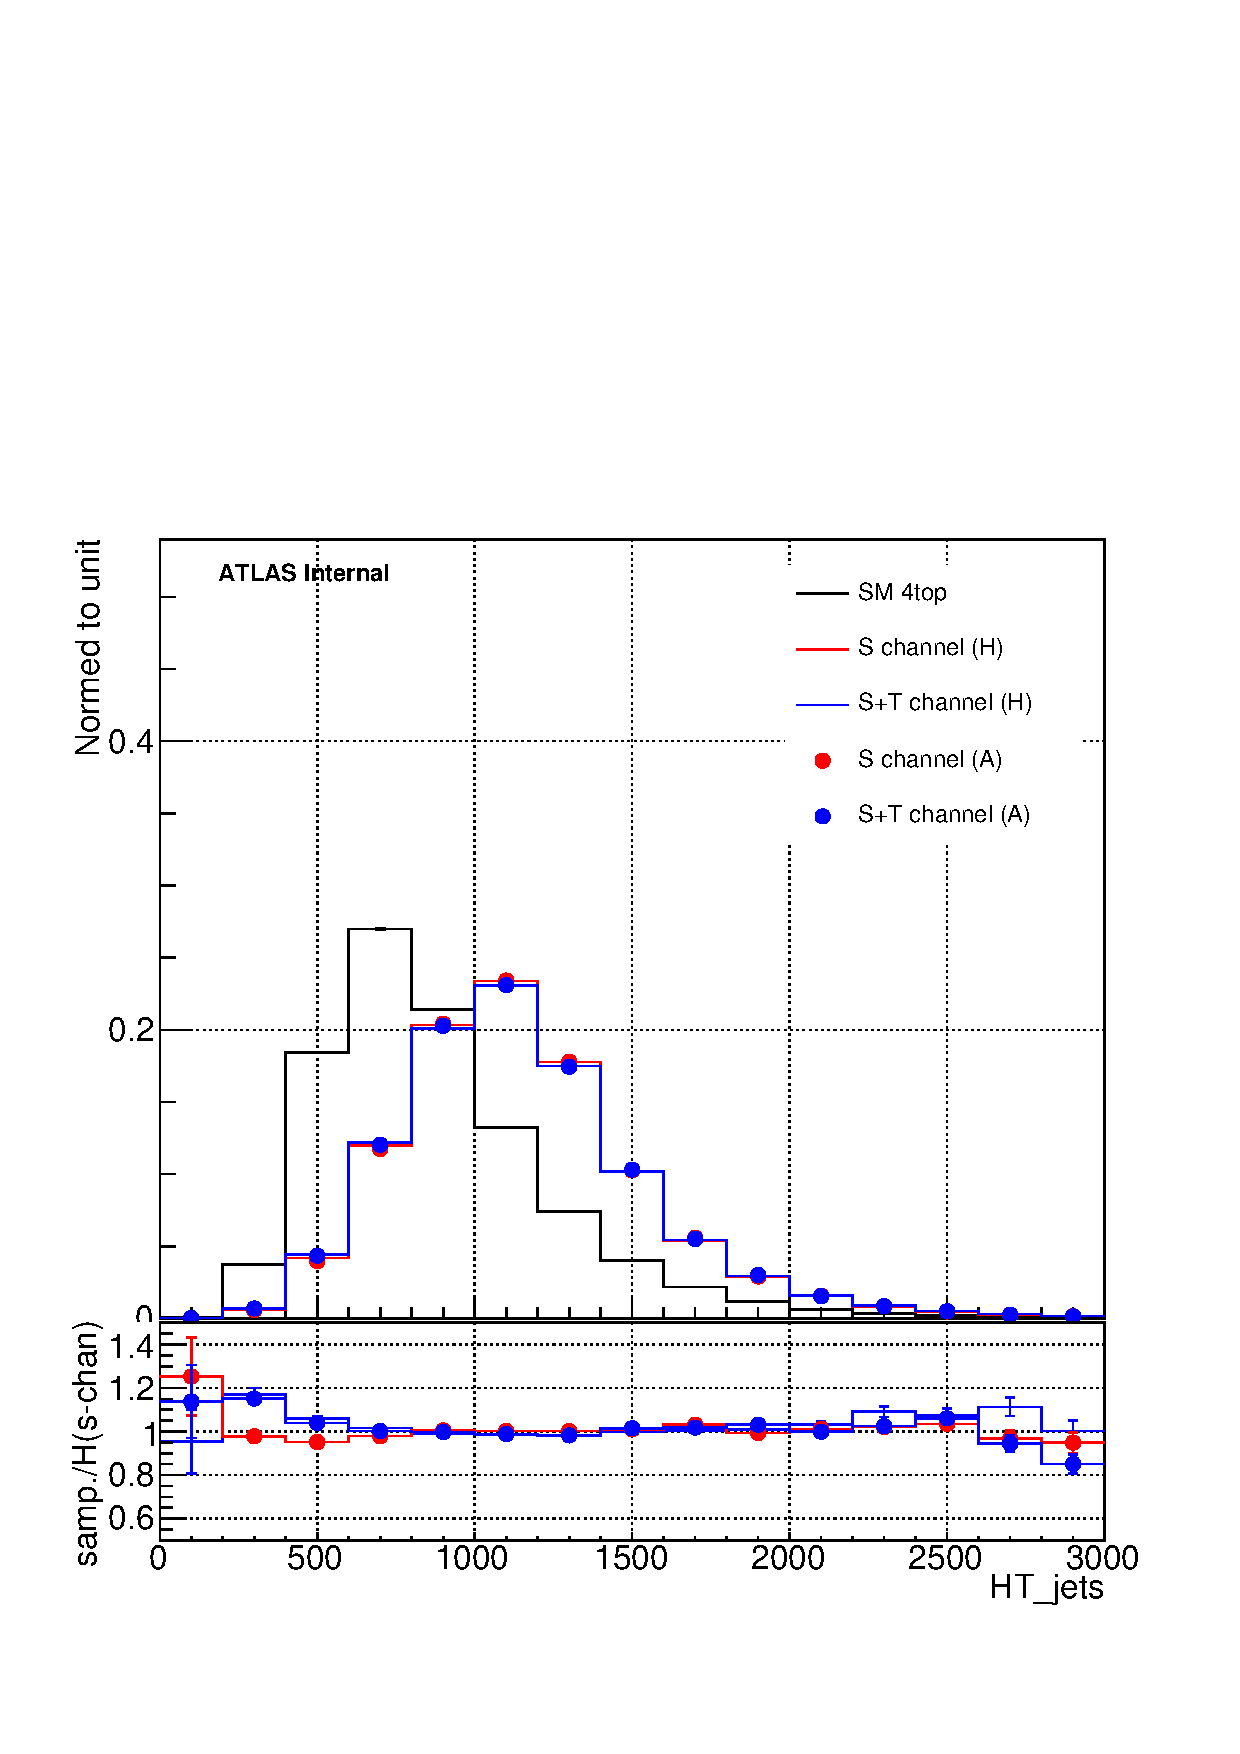
\includegraphics[width=0.9\linewidth]{figures/signal_modeling/HA_difference/Results_m1000_w30/Event_Inclusive_HT_jets_normed}
    \end{minipage}
  \begin{minipage}{0.33\textwidth}
    \centering
    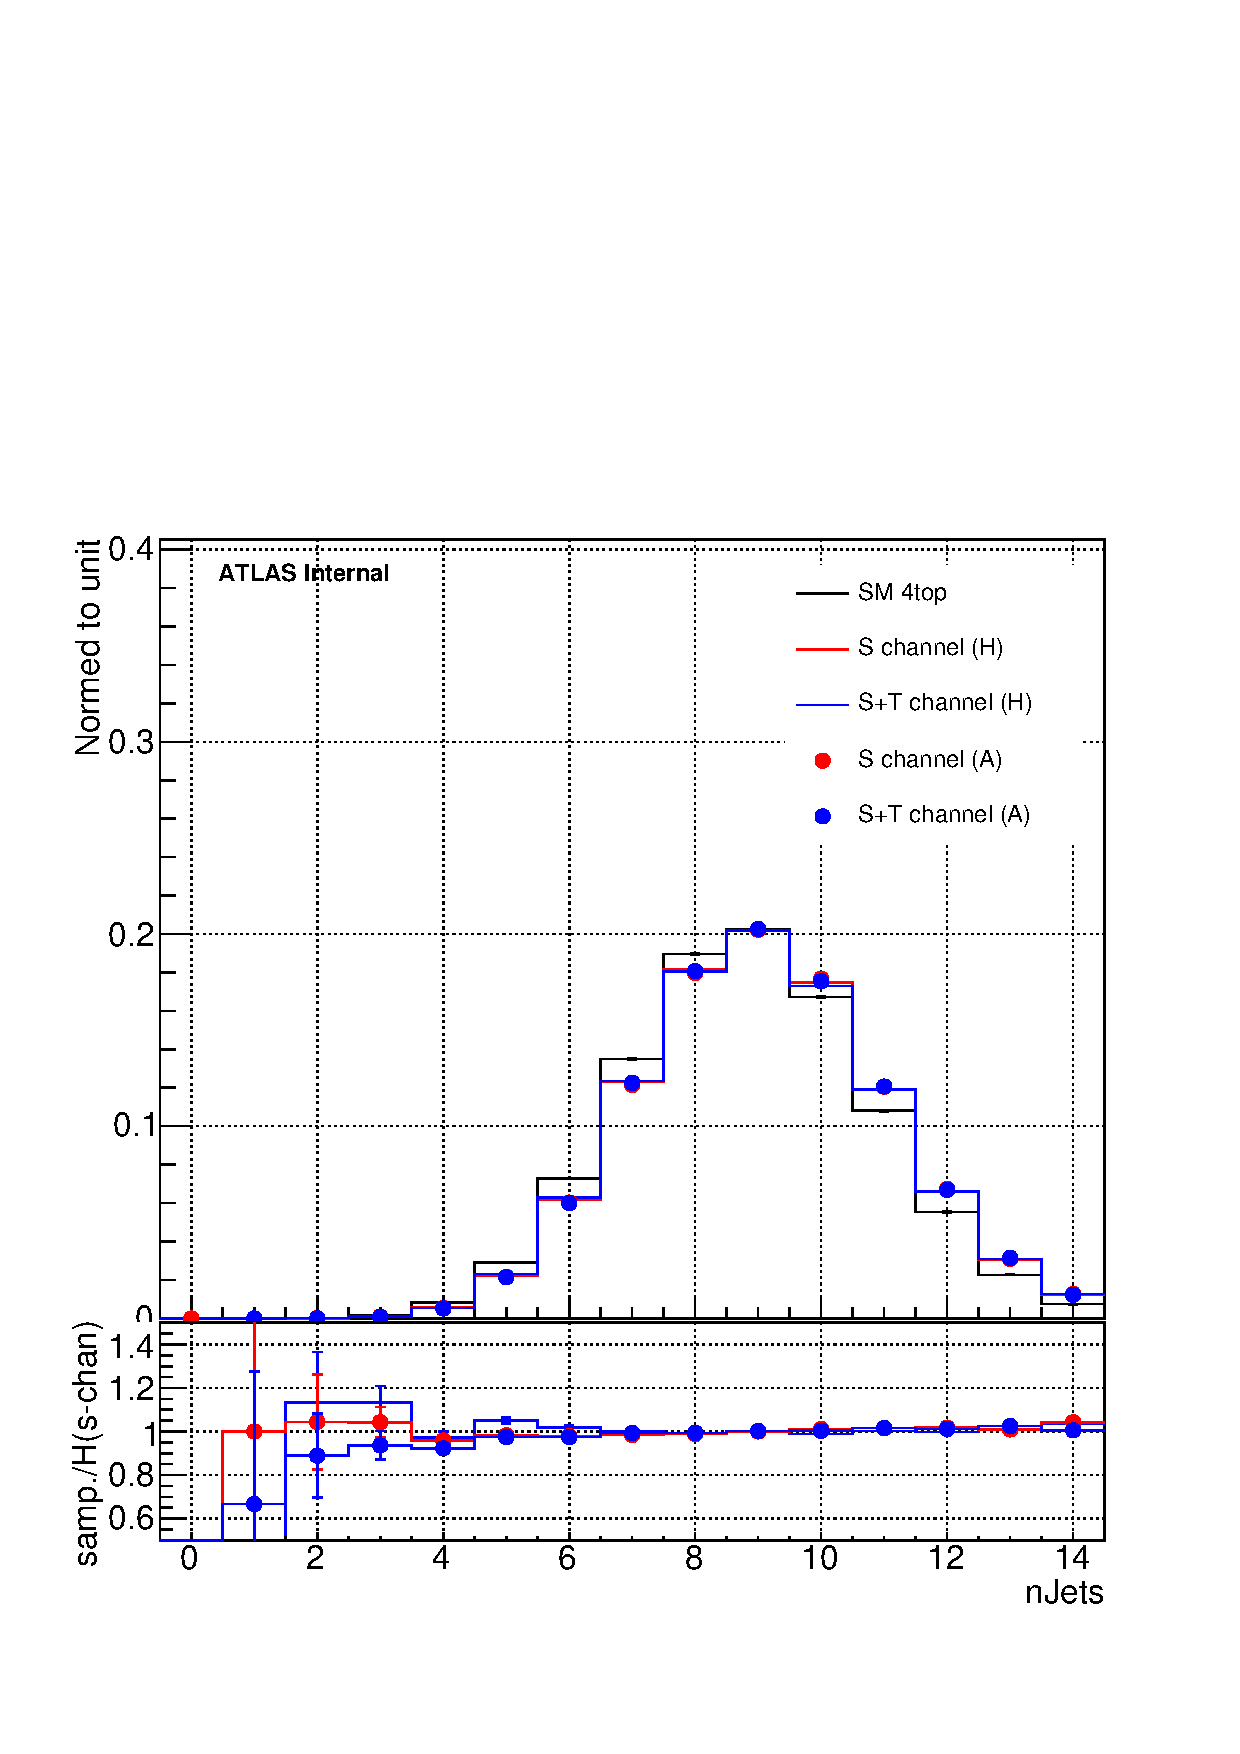
\includegraphics[width=0.9\linewidth]{figures/signal_modeling/HA_difference/Results_m1000_w30/Event_Inclusive_nJets_normed}
    \end{minipage}
  \begin{minipage}{0.33\textwidth}
    \centering
    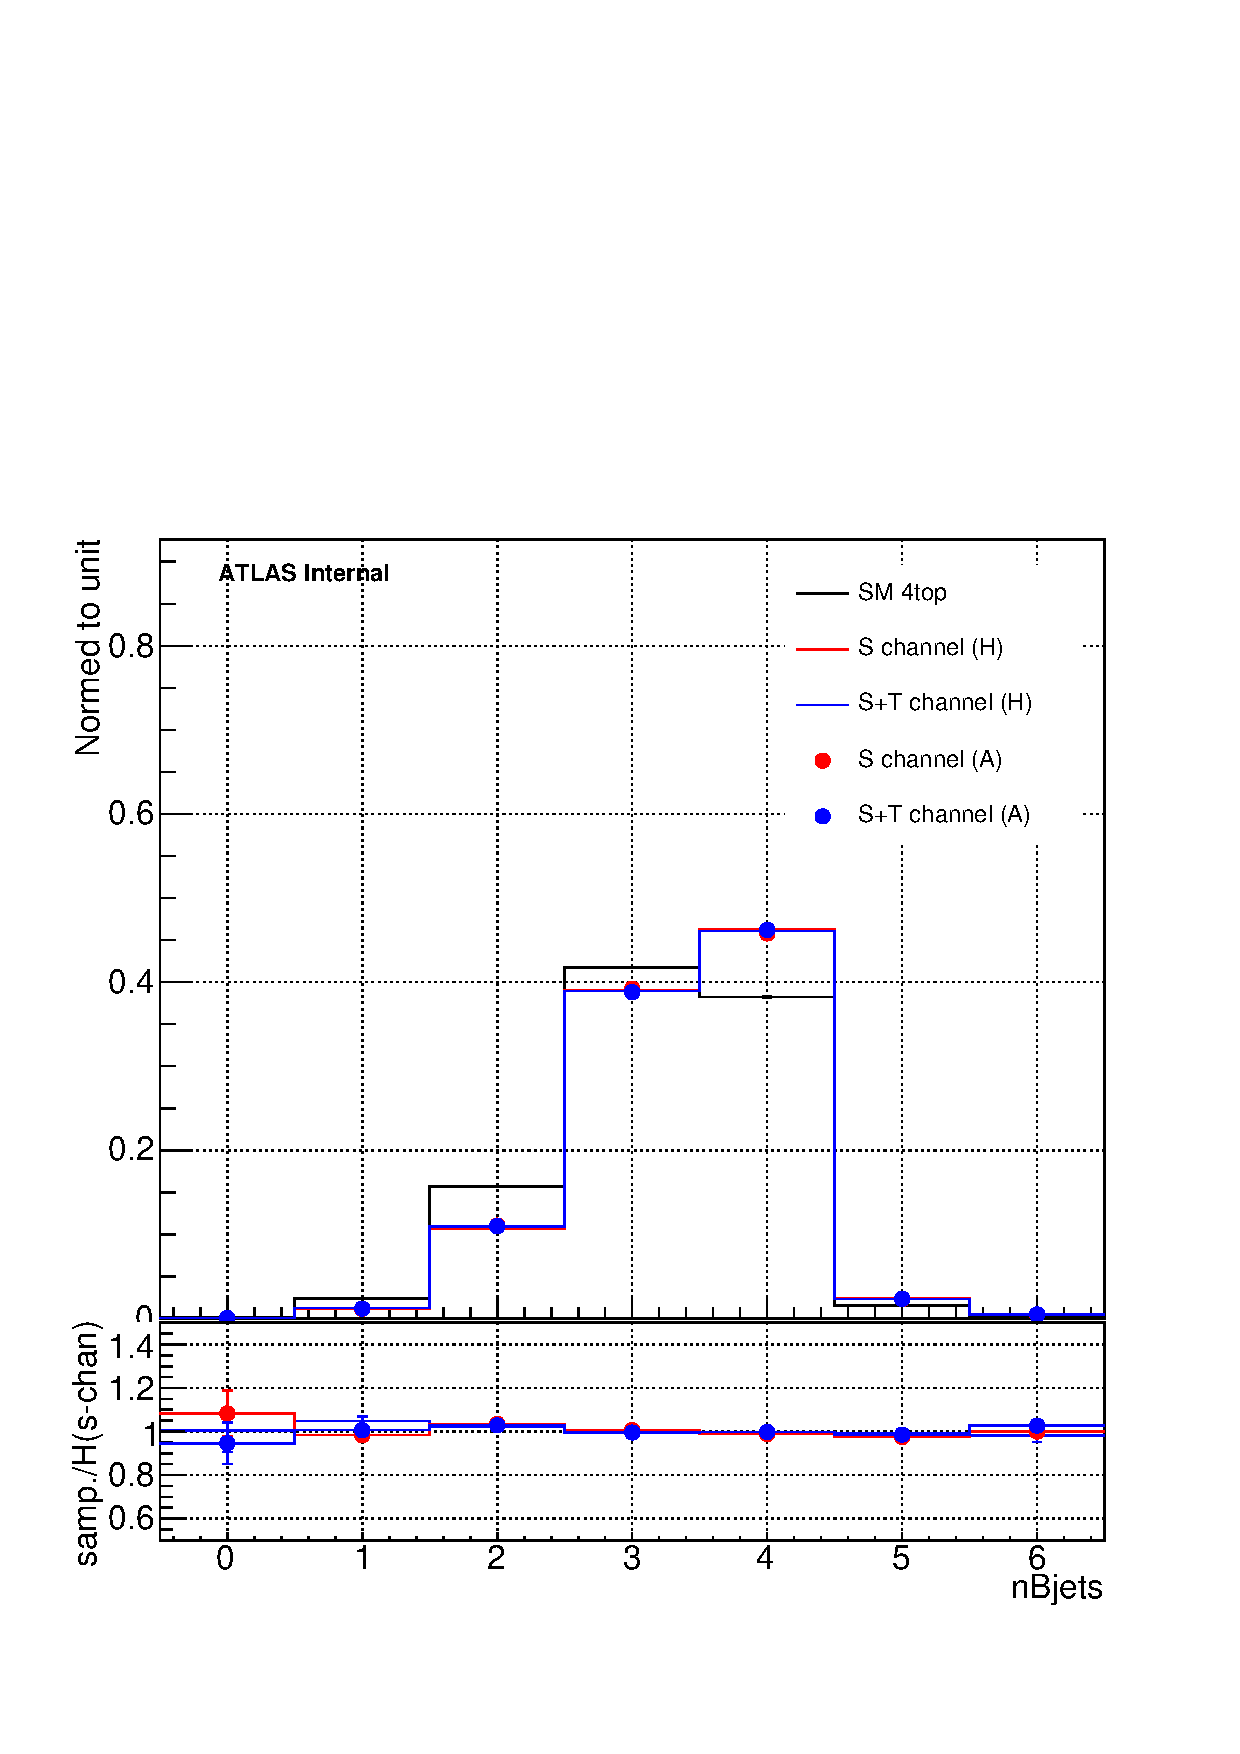
\includegraphics[width=0.9\linewidth]{figures/signal_modeling/HA_difference/Results_m1000_w30/Event_Inclusive_nBjets_normed}
    \end{minipage}
  \begin{minipage}{0.33\textwidth}
    \centering
    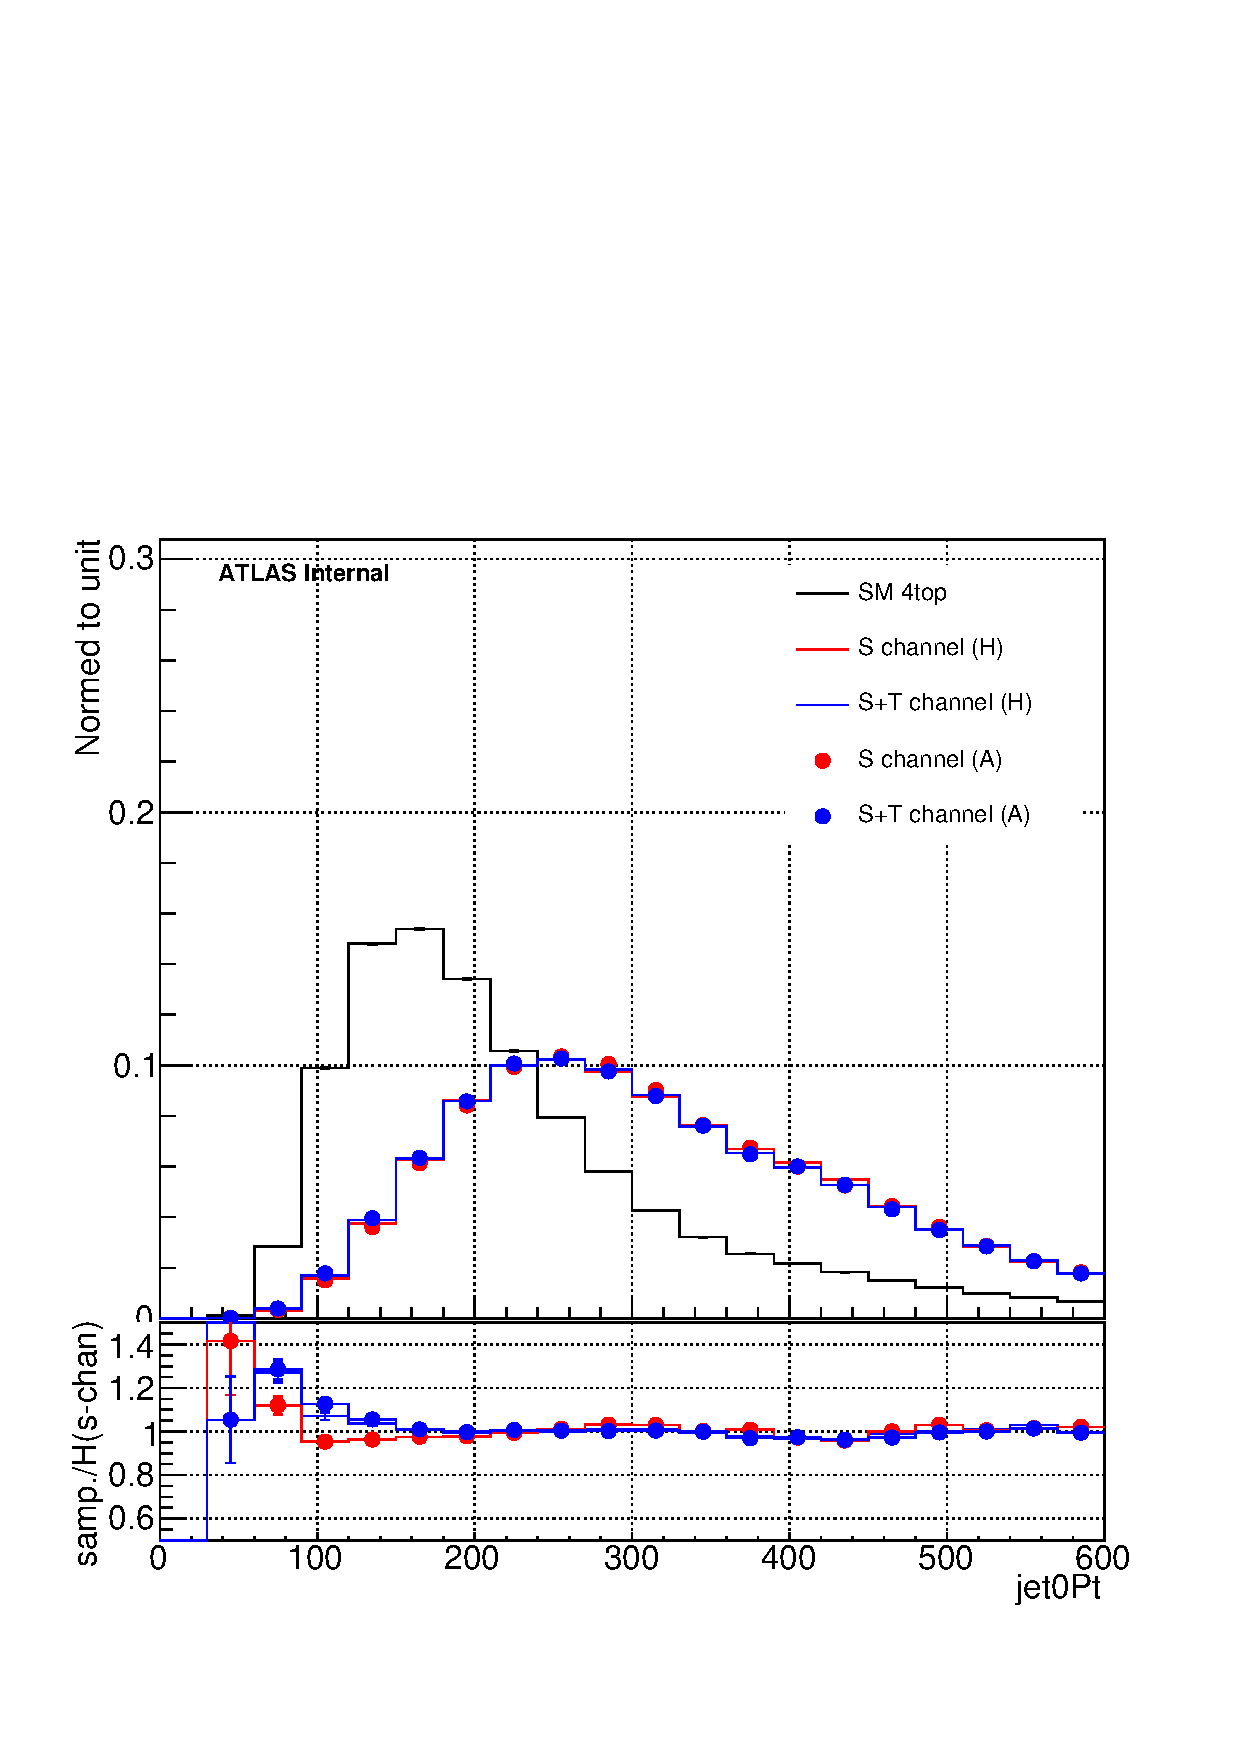
\includegraphics[width=0.9\linewidth]{figures/signal_modeling/HA_difference/Results_m1000_w30/Event_Inclusive_jet0Pt_normed}
    \end{minipage}
  \begin{minipage}{0.33\textwidth}
    \centering
    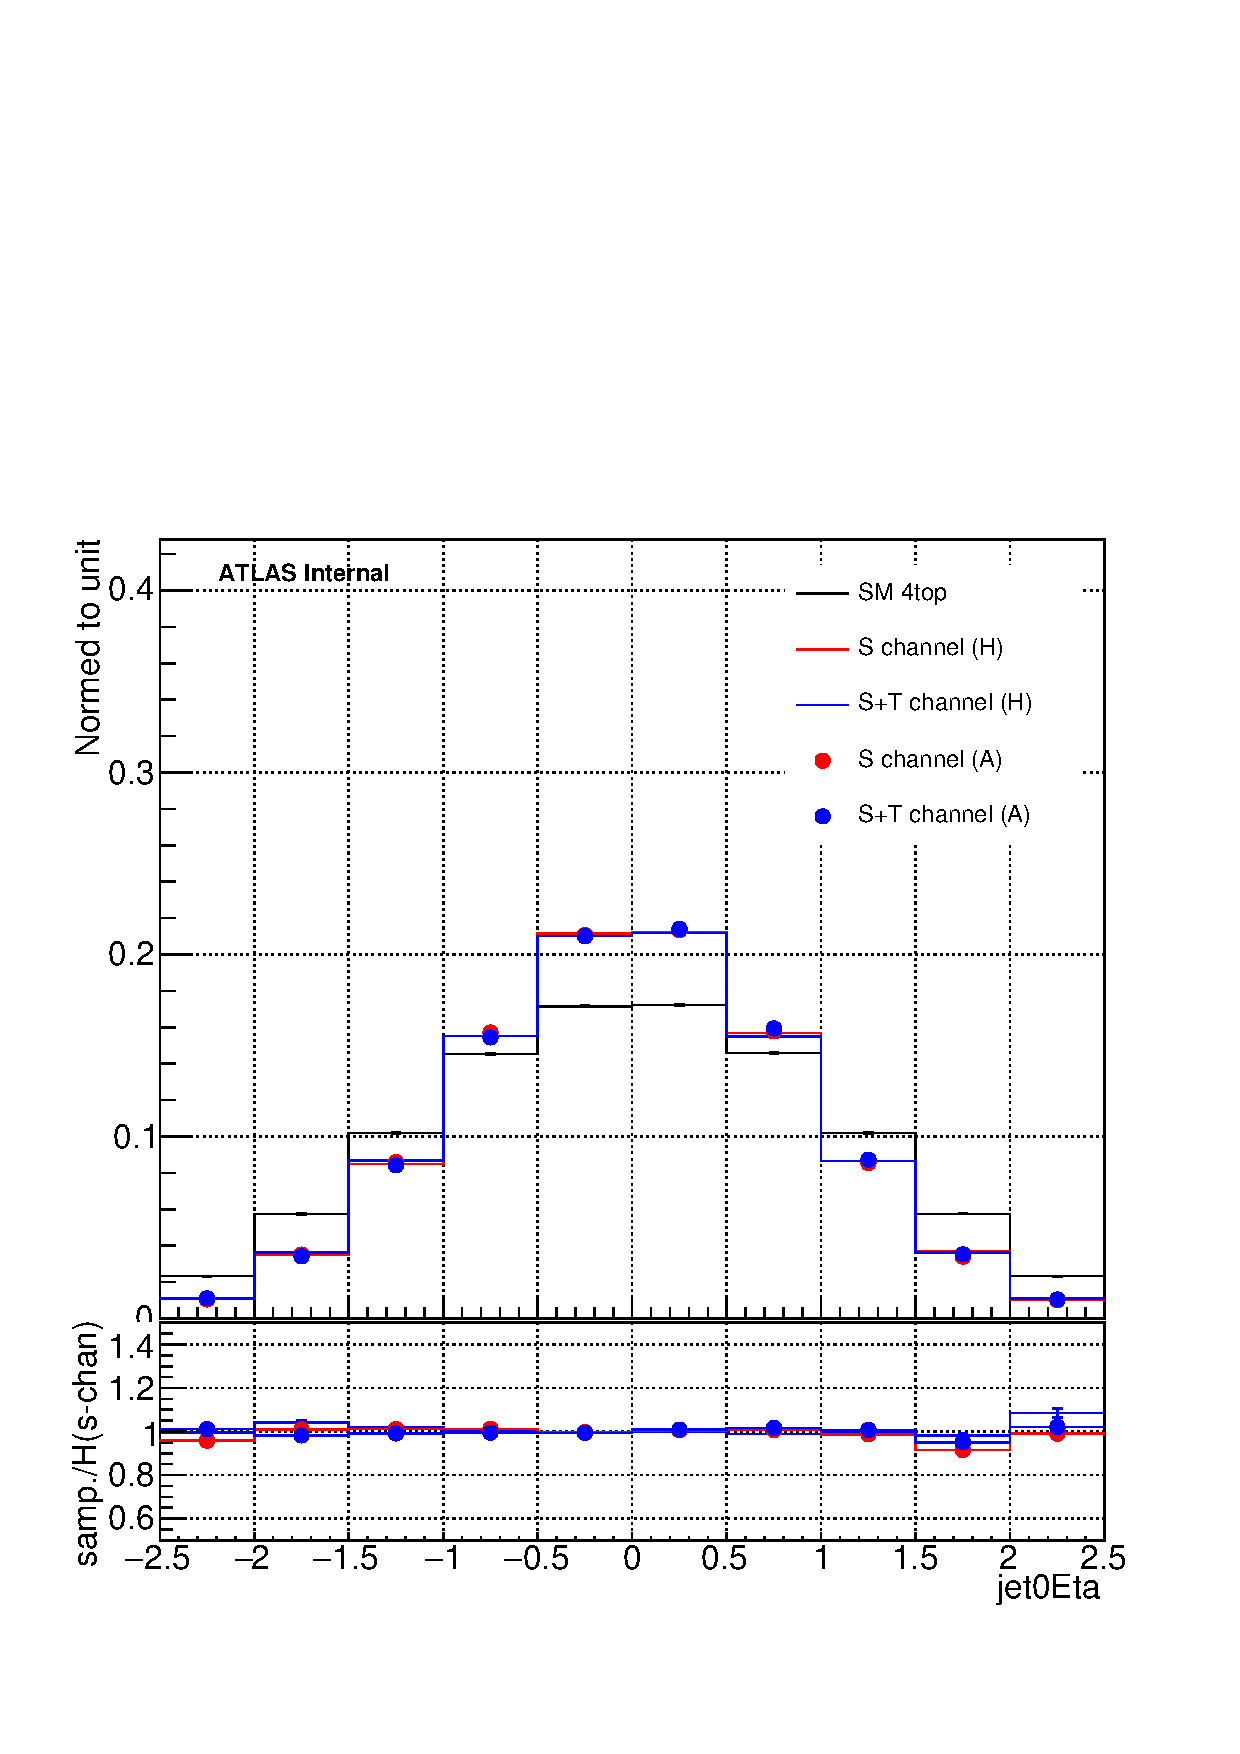
\includegraphics[width=0.9\linewidth]{figures/signal_modeling/HA_difference/Results_m1000_w30/Event_Inclusive_jet0Eta_normed}
    \end{minipage}
  \begin{minipage}{0.33\textwidth}
    \centering
    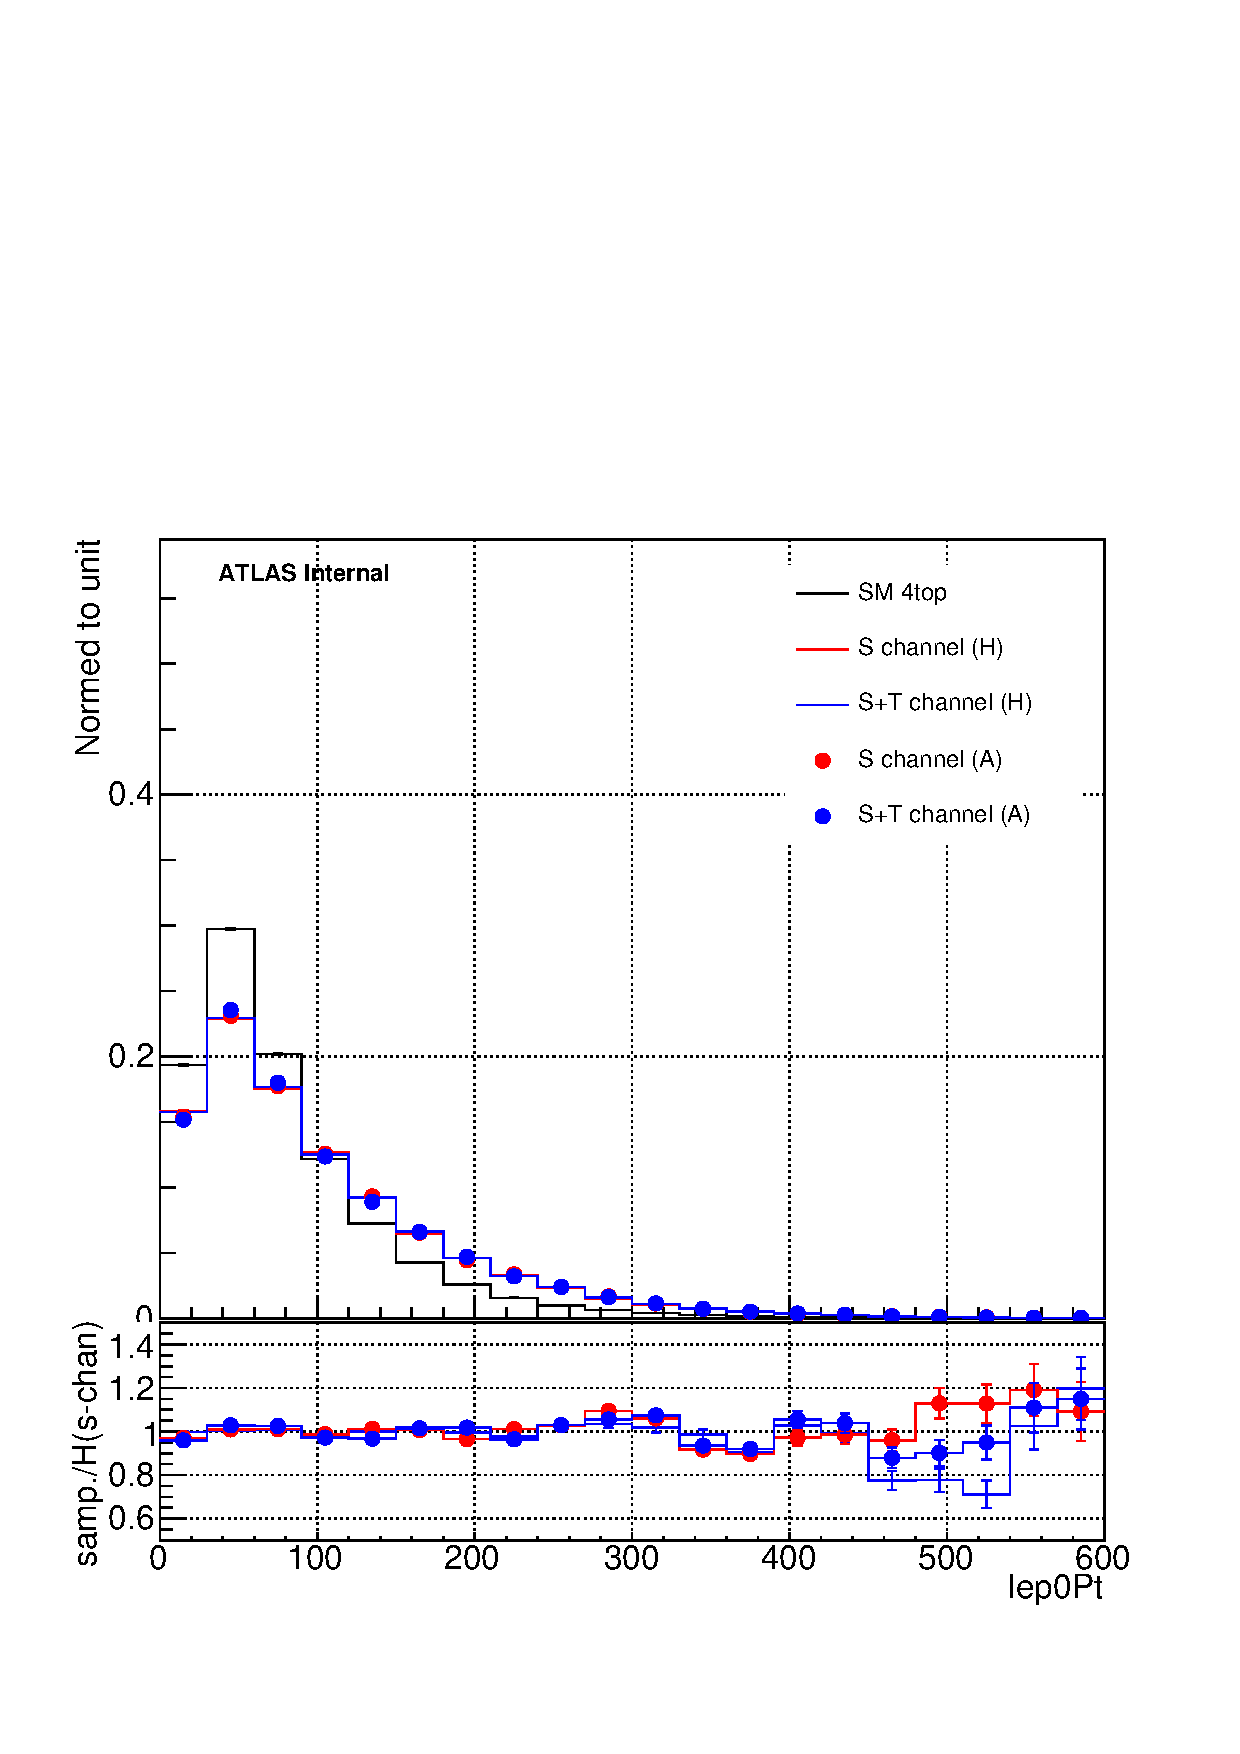
\includegraphics[width=0.9\linewidth]{figures/signal_modeling/HA_difference/Results_m1000_w30/Event_Inclusive_lep0Pt_normed}
    \end{minipage}
  \begin{minipage}{0.33\textwidth}
    \centering
    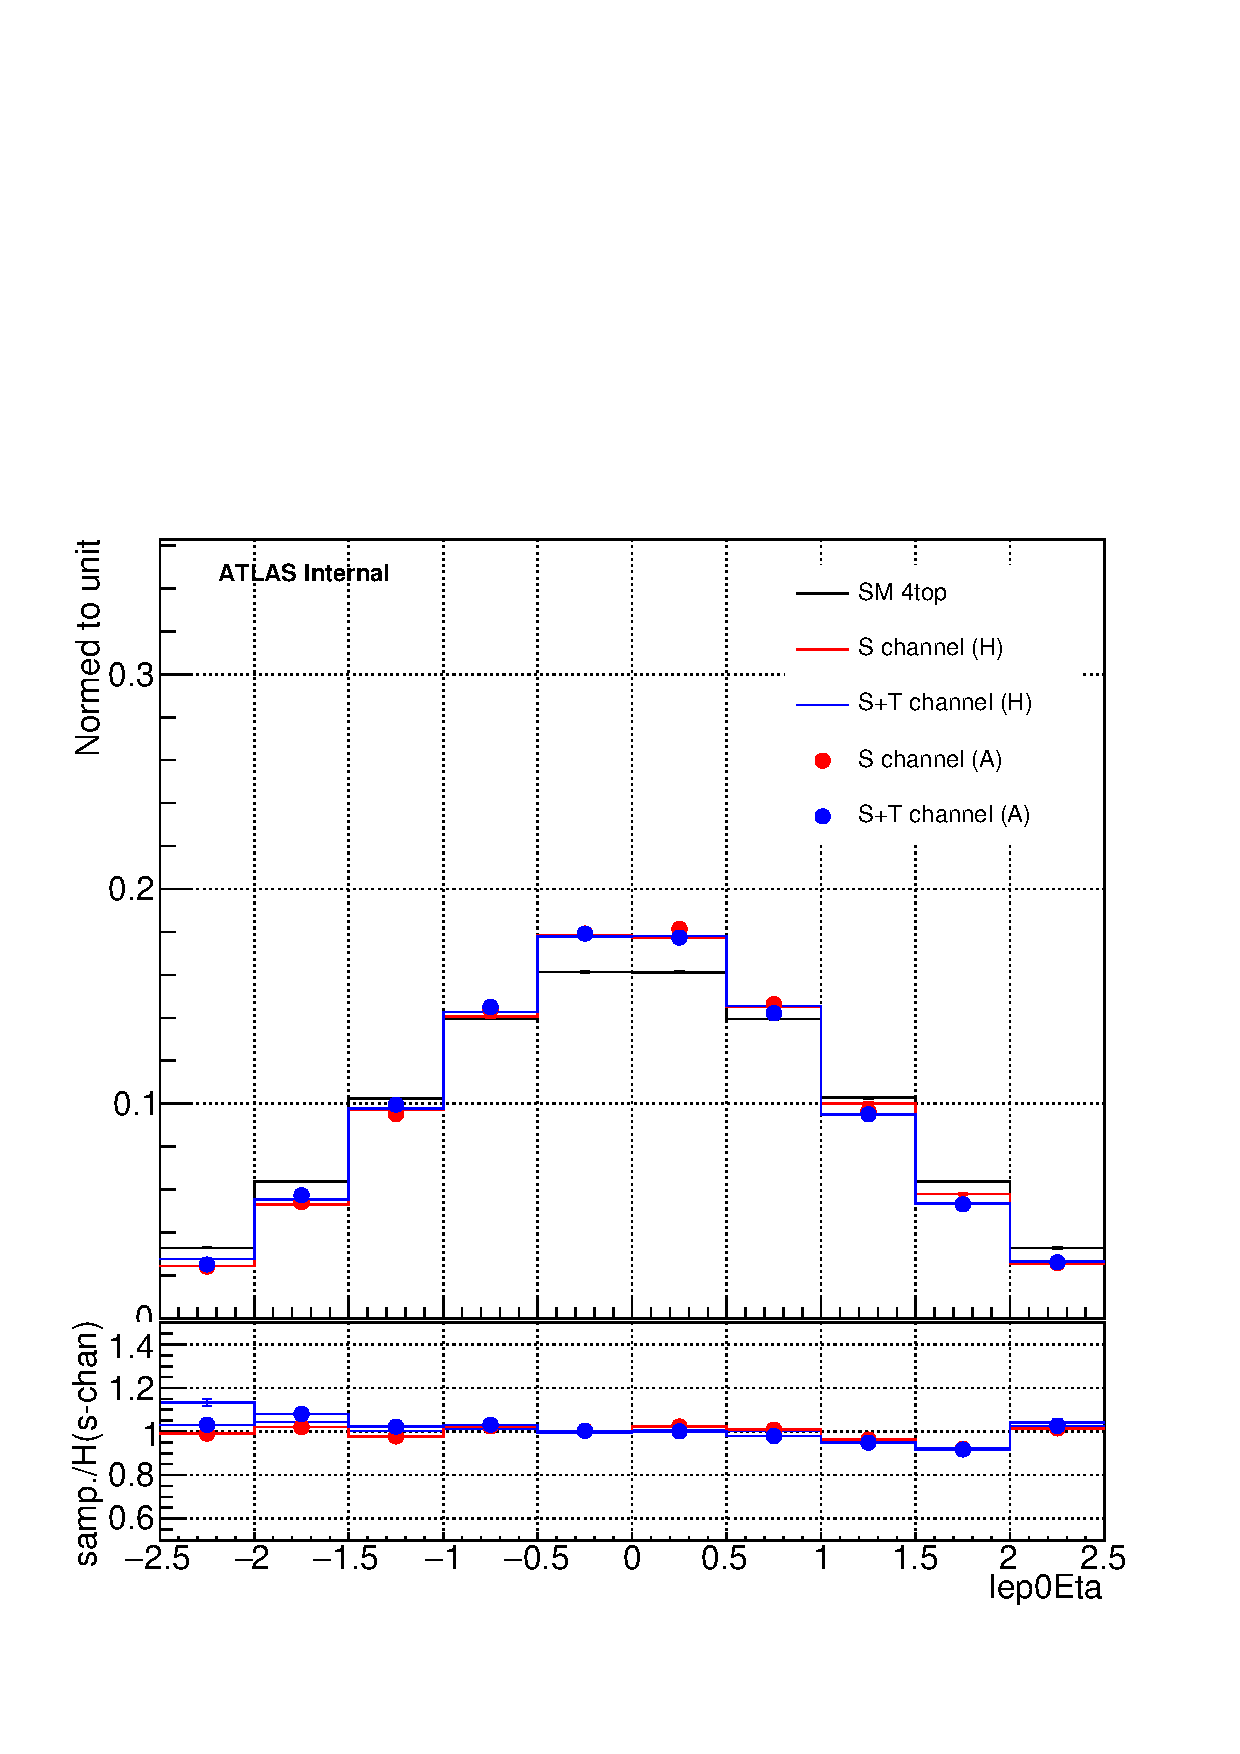
\includegraphics[width=0.9\linewidth]{figures/signal_modeling/HA_difference/Results_m1000_w30/Event_Inclusive_lep0Eta_normed}
    \end{minipage}
  
  \caption{\label{Fig:t_channel_1000}Kinematic comparison between $t\bar{t}H$ and $t\bar{t}A$ production in the $s$-channel and $s$+$t$-channel for $\mH=1000$~GeV in the inclusive region. The shapes are normalised to unit.}

\end{figure}
